% poster.pdf（A1 で組んだ版面）を A0 縦（841 × 1189 mm）に拡大する。
% ベクターのまま拡大するので、文字や図は粗くならない。
% A1 と A0 の縦横比は 0.1% だけ違うので、高さを合わせて左右に 0.6 mm ずつ余白ができる。
% 先に poster.tex をビルドしておくこと（build_poster.bat が両方を順にビルドする）
\documentclass{article}
\usepackage[paperwidth=841mm,paperheight=1189mm,margin=0mm]{geometry}
\usepackage{graphicx}
\pagestyle{empty}
\setlength{\parindent}{0pt}
\setlength{\topskip}{0pt}
\begin{document}
\makebox[\linewidth][c]{\raisebox{-\height}[0pt][0pt]{%
  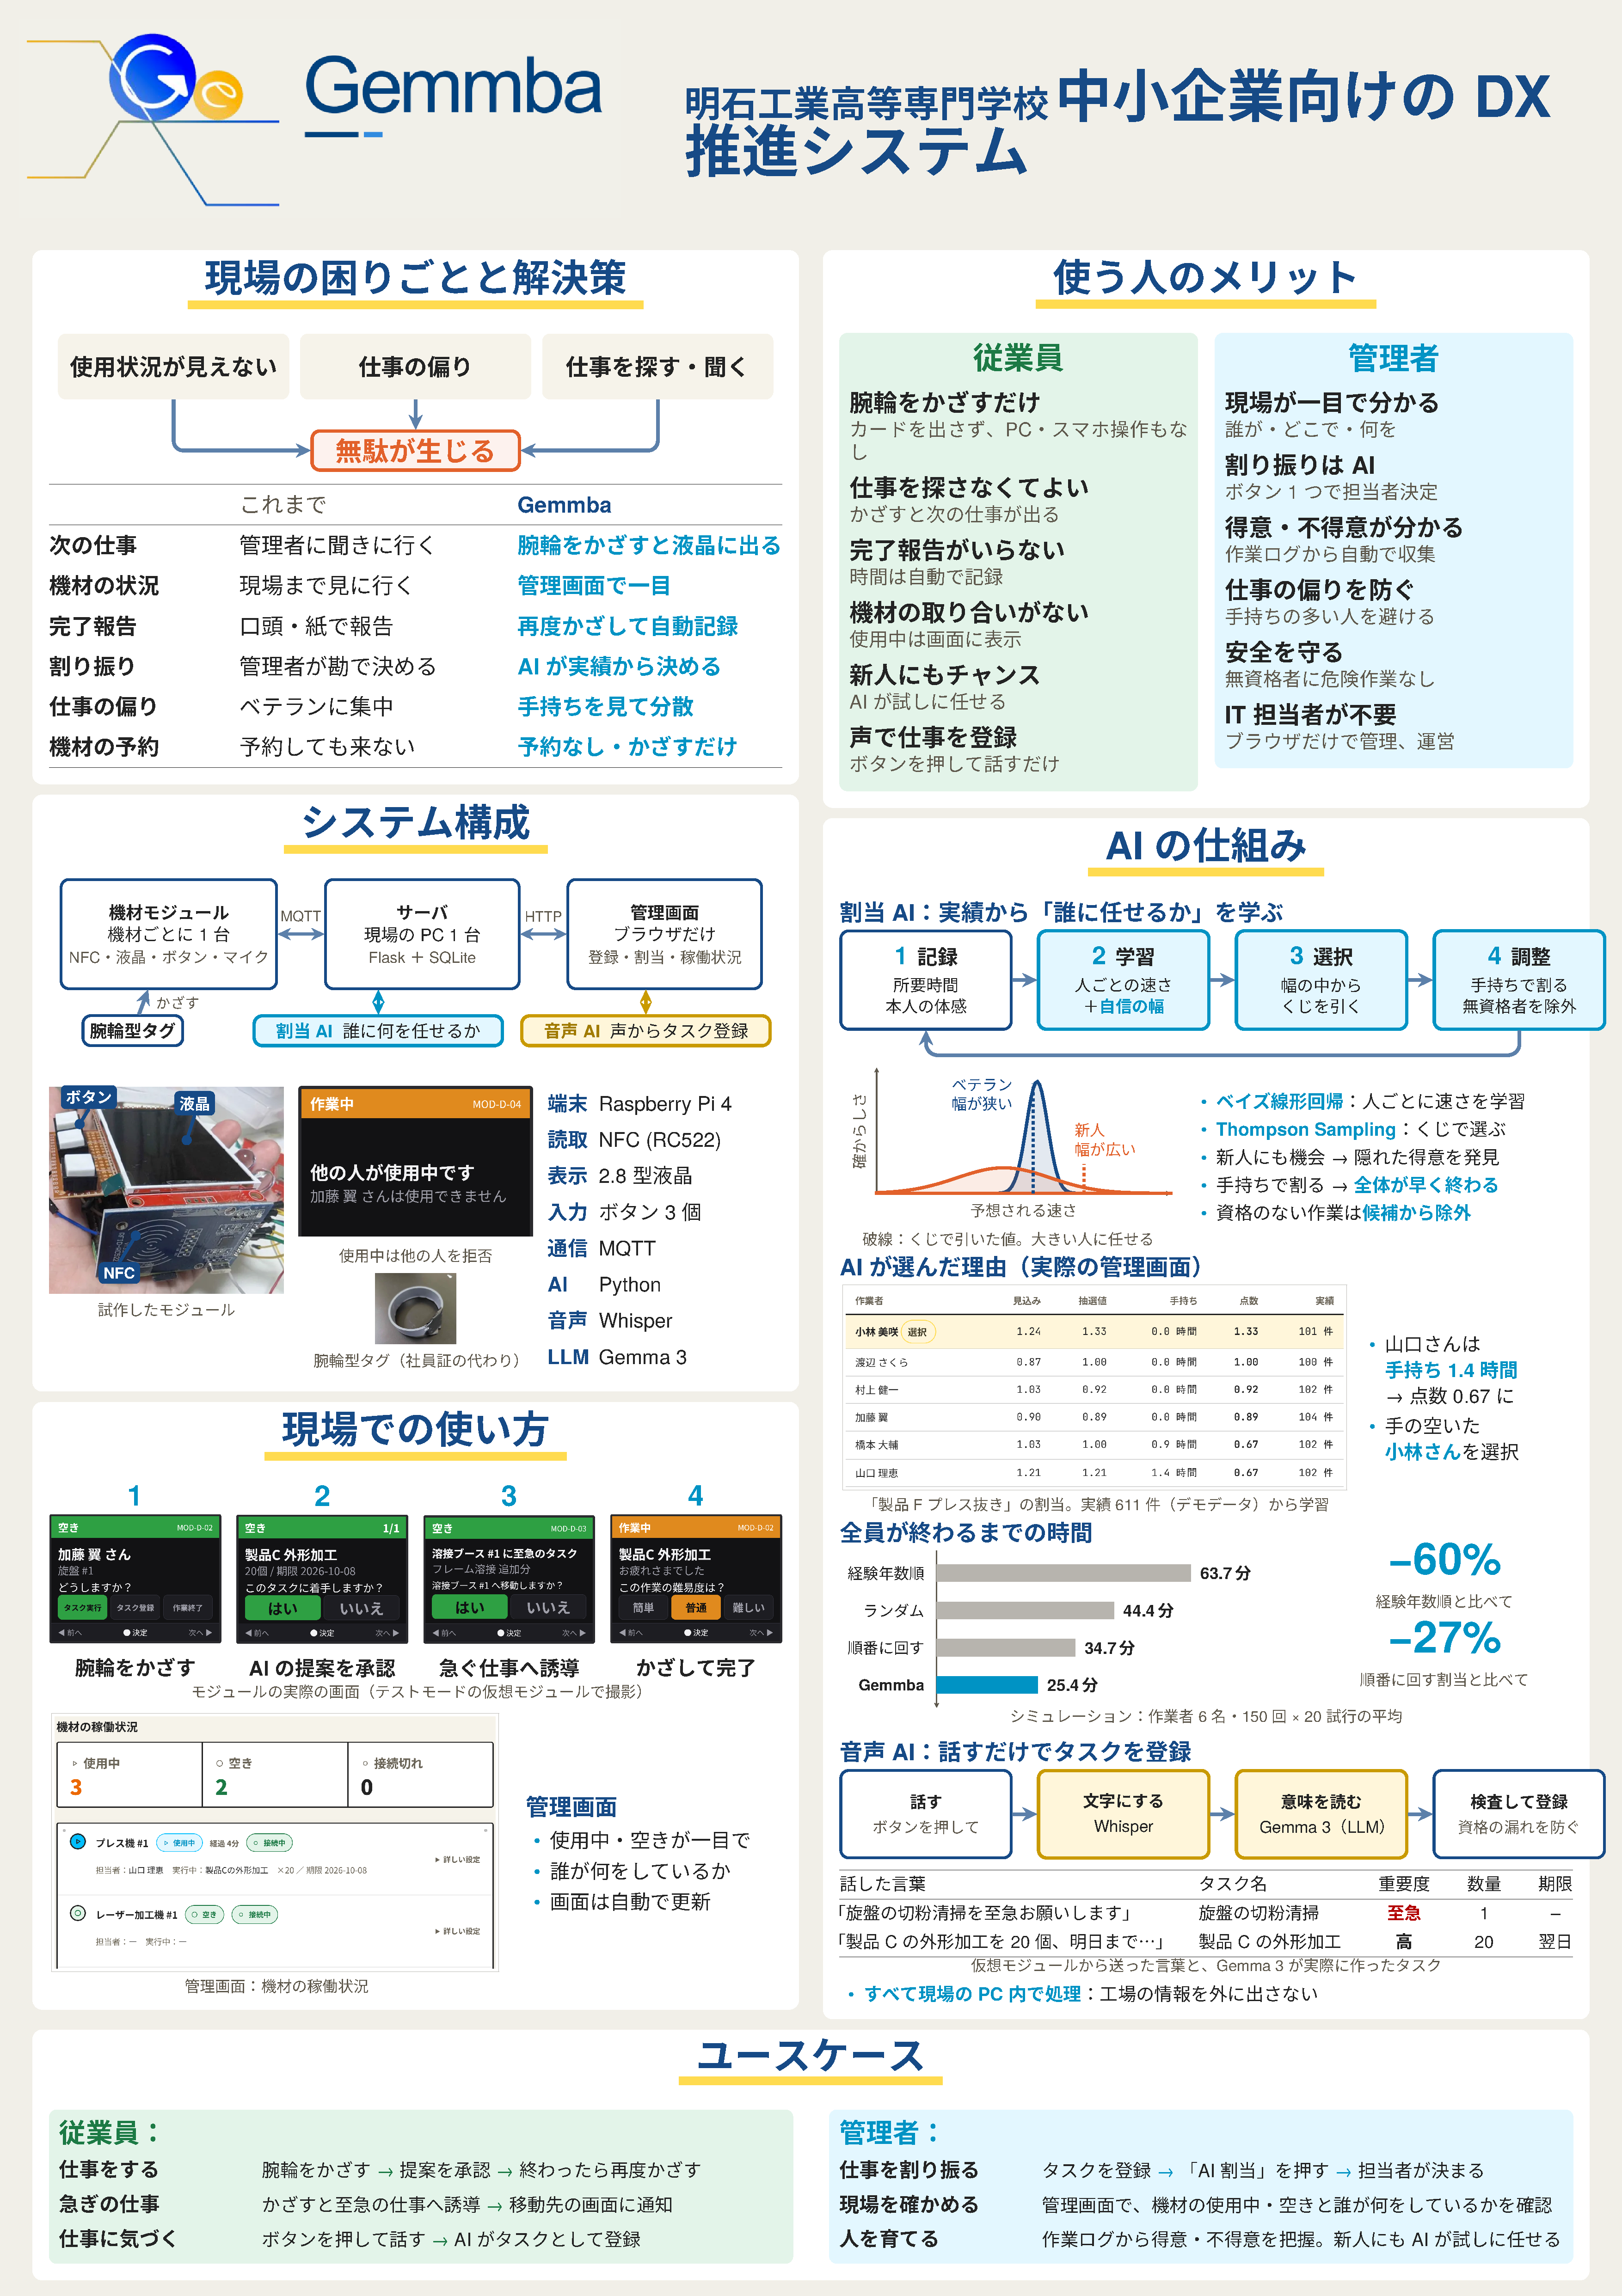
\includegraphics[height=1189mm,keepaspectratio]{poster.pdf}}}
\end{document}
